\section*{Part E}
\addcontentsline{toc}{section}{Part E}

\begin{tcolorbox}
  E.1) For the wave in equation 15, listen to harmonics 1, 2 and 3 individually then as a chord. Plot the chord waveform as well. Provide the Matlab code used to listen to the harmonics/chord and plot the chord.
\end{tcolorbox}

\lstinputlisting[
  caption = Requirement 1 MATLAB code,
  label = code:E_r_1,
]{matlab/E_r_1.m}

\begin{figure}[htbp]
  \centering
  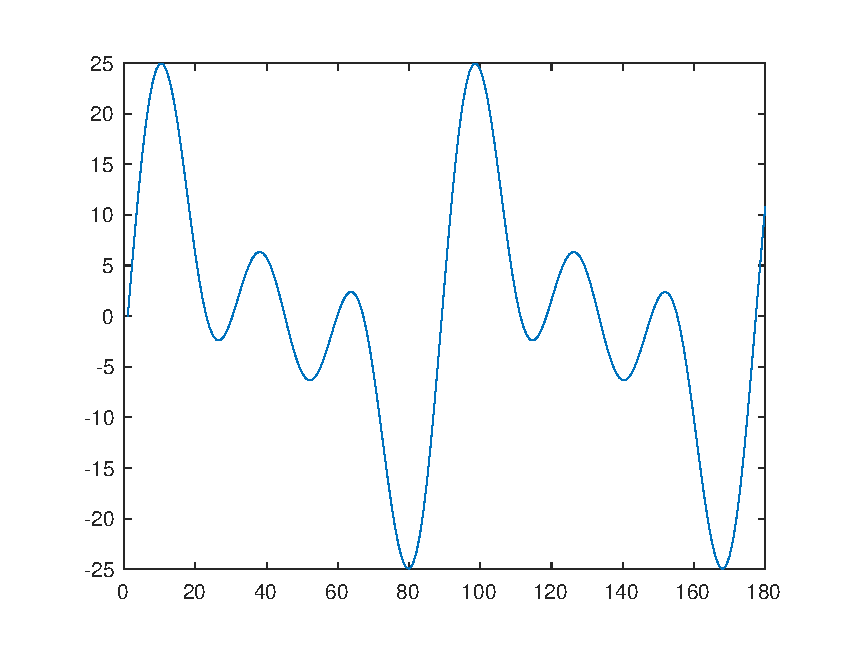
\includegraphics [width=4in]{matlab/fig/E_r_1.eps}  
  \caption{chord $V(t)=10[\sin(2\pi f_o t)+\sin(2\pi 2f_o t)+\sin(2\pi 3f_o t)]$ with a fundemental frequncy $f_o=500Hz$}    
  \label{fig:E_r_1}
\end{figure}

\begin{tcolorbox}
  E.2) Alter the phase of the third harmonic in equation 15 by 90◦ and repeat the tasks in the point above.
\end{tcolorbox}

\lstinputlisting[
  caption = Requirement 2 MATLAB code,
  label = code:E_r_2,
]{matlab/E_r_2.m}

\begin{figure}[htbp]
  \centering
  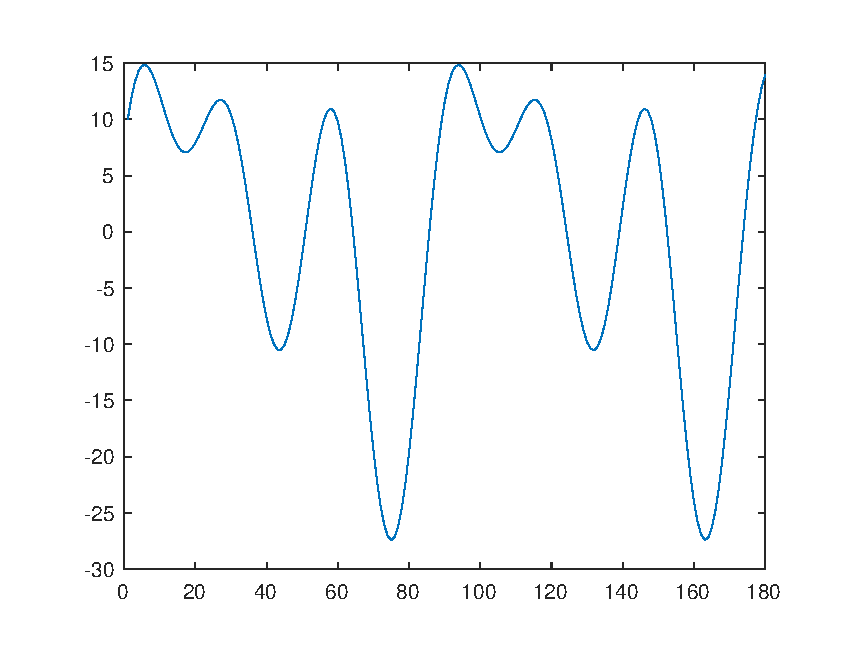
\includegraphics [width=4in]{matlab/fig/E_r_2.eps}  
  \caption{The third harmonic of the chord of Figure \ref{fig:E_r_1} is shifted by 90\textdegree.}
  \label{fig:E_r_2}
\end{figure}

\begin{tcolorbox}
  E.3) Discuss the effect of altering the phase of the third harmonic, both on the sound and plot of the chord. Do the sound or plot change as you alter the phase? Why?
\end{tcolorbox}

The plot of chord is changed but sound does not. This is because timbre depends primarily upon the frequency spectrum, not the shape of the signal in time domain.

\begin{tcolorbox}
  E.4) What does the above tell you about the human ear?
\end{tcolorbox}

Human ear can distinguish different sounds by frequency and combination of them. However, human ear cannot identify the difference between signals which have same spectrum but different phase of each corresponding hamonics.

\pagebreak